% Metoddelen redogör för vad du gjort och hur du gått tillväga; det är
% en beskrivning av den metod som ligger till grund för det du kommit
% fram till och hävdar i din rapport.

% Beskrivningen i metoddelen ska vara koncis snarare än helt
% uttömmande men ska samtidigt göra det möjligt att upprepa studien

% Metoddelen ska inte vara en omgjord labbinstruktion och den ska inte
% heller innehålla teori med mindre än att teoretiska hänsyn har haft
% en direkt inverkan på metoden.

% Metoddelen skrivs nästan alltid i dåtid (imperfekt) och ofta används
% passiv form för att beskriva forskningsaktiviteter.

\chapter{Genomförande}

Projektets genomförande bestod av fyra delar. Den största delen var
konstruktionen av själva läromaterialet, och där ingick sökande efter fysikaliska
områden, implementation av domänspecifika språk och skrivande av lärotext. De
tre andra delarna var publicering av läromaterialet på en hemsida, utvärdering
av läromaterialet med en testgrupp samt möten med Åke Fäldt, examinator och
föreläsare för Fysik för ingenjörer. Mötena med Fäldt hade två syften: att hitta
problemområden i fysikkursen och att få återkoppling på läromaterialet. Alla de olika delar i projektet genomfördes samtidigt men de finns här beskrivna separat.

\section{Konstruktion av läromaterialet}\label{sec:konstruktion}

Läromaterialet består av 5 kapitel som vardera behandlar separata
områden. Skapandet av varje kapitel skedde därför till största delen fristående
från andra kapitel. Skapandet av kapitlena bestod i sin tur av tre faser,
som såg likadana ut för alla kapitel. Dessa faser var sökande efter område,
implementation av domänspecifika språk för området samt skrivande av lärotext.

Denna skapandeprocess kan delas upp i en graf med två axlar: en utefter kapitel
och en utefter fas. Det här illustreras i figur~\ref{fig:oversiktA}. Figuren
visar att varje kombination av kapitel och fas är en del i projektet som
arbetades med.

\begin{figure}[tph]
    \centering
    \begin{subfigure}[t]{0.5\textwidth}
        \centering
        \frame{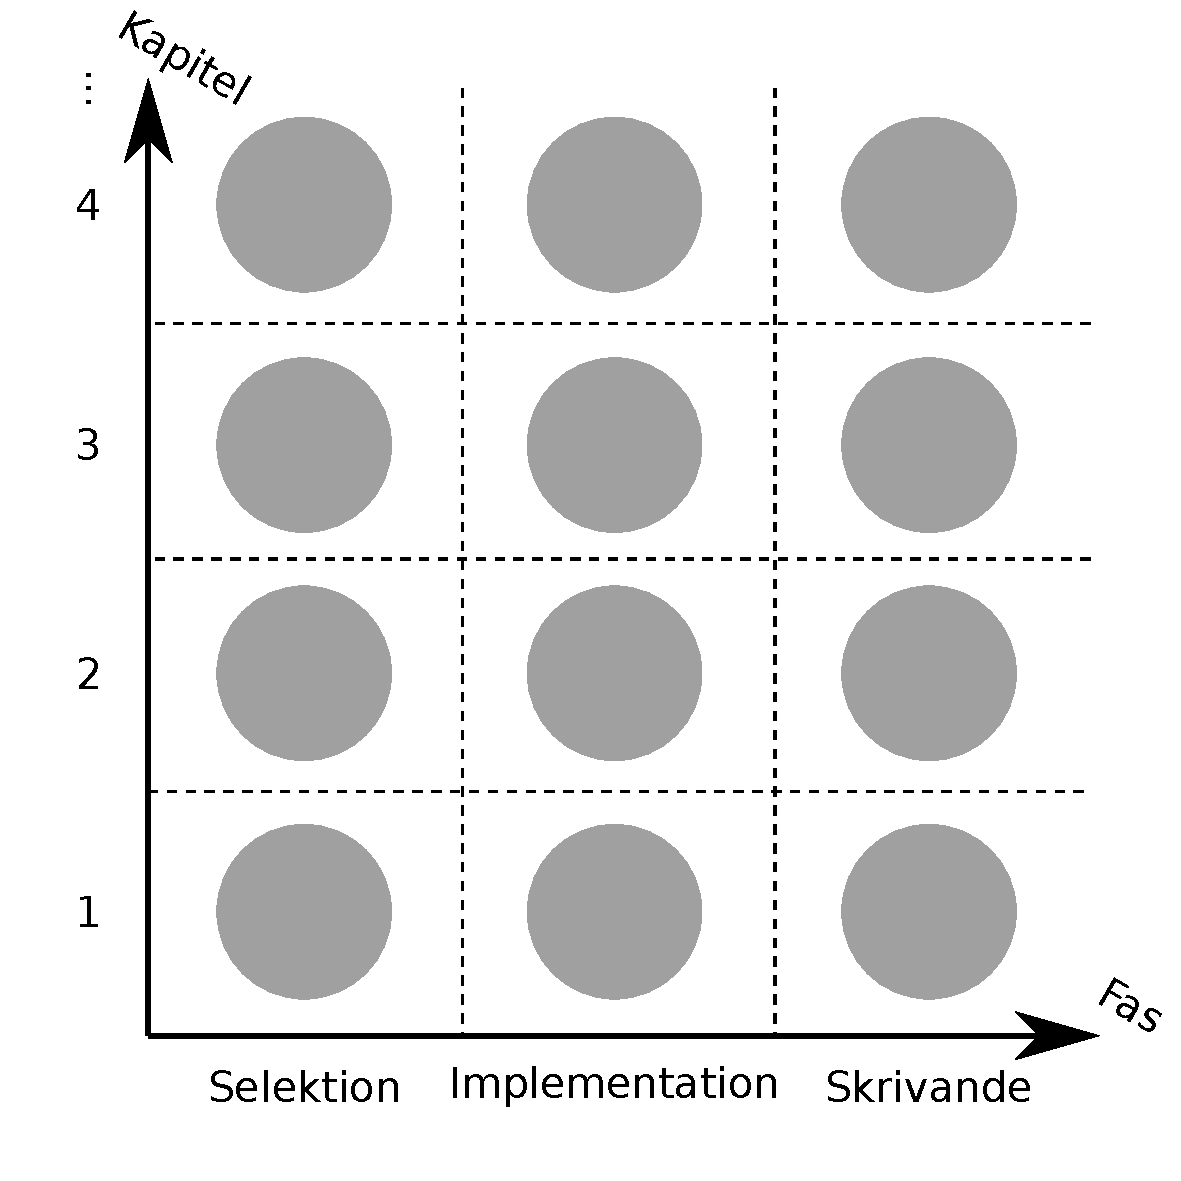
\includegraphics[width=0.9\linewidth]{figure/oversiktA.pdf}}
        \caption{Delarna visas distinkta och var för sig.}\label{fig:oversiktA}
    \end{subfigure}% <- This comment makes the figure lie side by side ¯\(°_o)/¯
    ~~~
    \begin{subfigure}[t]{0.5\textwidth}
        \centering
        \frame{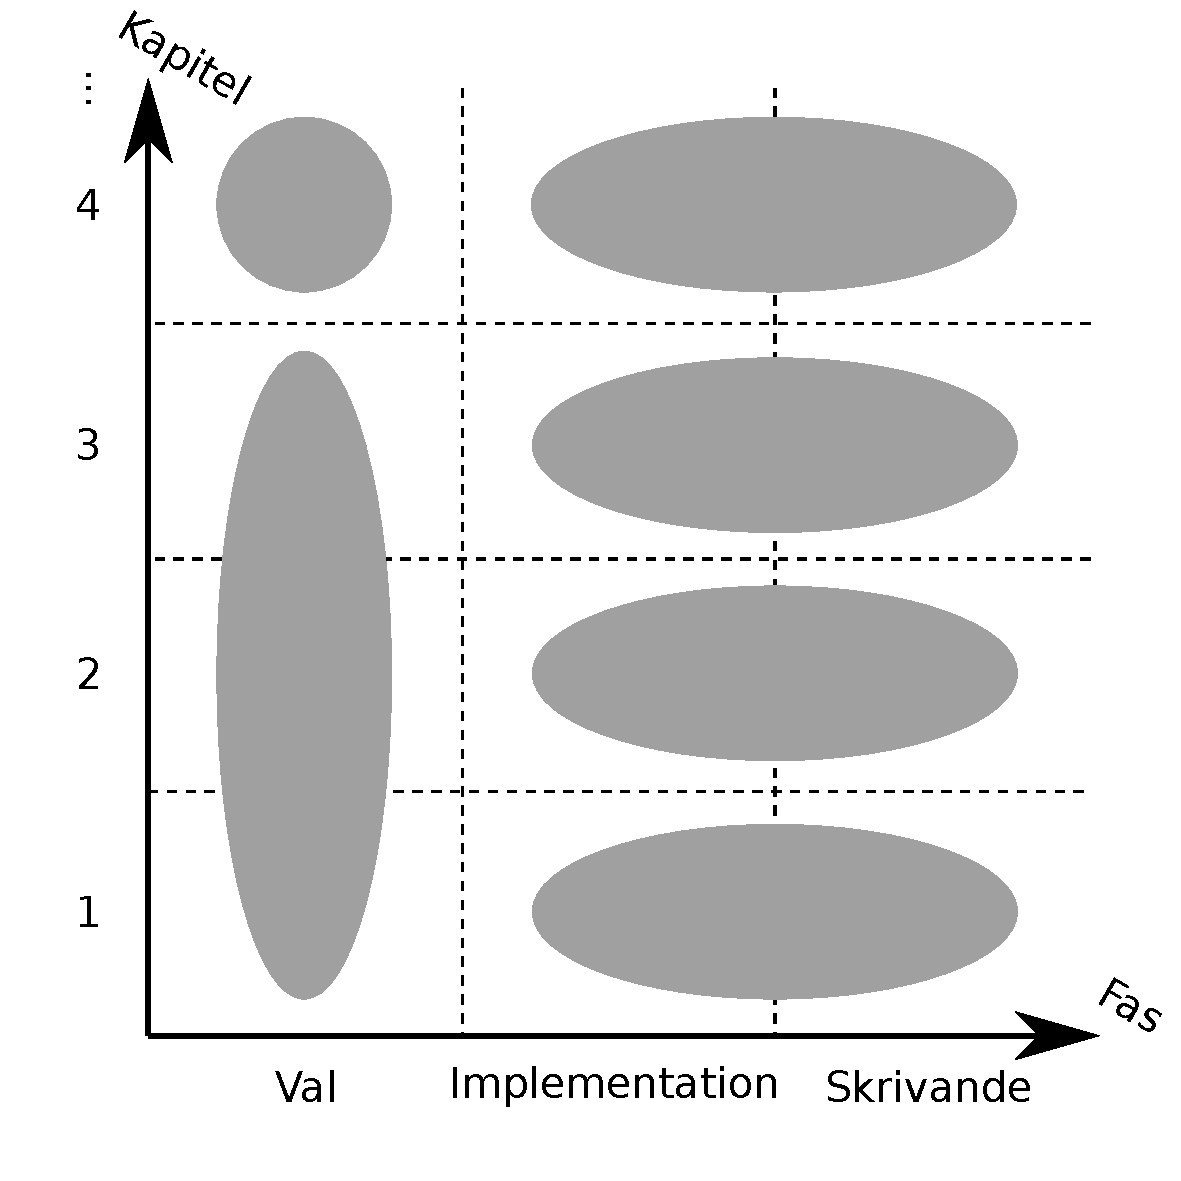
\includegraphics[width=0.9\linewidth]{figure/oversiktB.pdf}}
        \caption{Delarna visas med gränsöverskridande överlapp. Notera att
        implementation och skrivande \textit{alltid} var överlappande medan
      sökande \textit{ofta men inte alltid} var det.}~\label{fig:oversiktB}
    \end{subfigure}
    \caption{Översikt över hur skapandeprocessen av läromaterialet såg ut.
  Processen delas upp utefter två axlar: kapitel och fas. Varje kombination
  är en del som arbetats med och är gråmarkerad.} 
\end{figure}

Även om detta sätt att dela upp processen är översiktligt är det inte helt
verklighetstroget. I praktiken fanns det överlapp mellan de olika delarna, både
med avseende på kapitel och fas. Det här illustereras i
figur~\ref{fig:oversiktB}. Där ser man att sökandet av områden skedde för flera
kapitel samtidigt. Detta då arbetet med att hitta ett område ofta gav flera
områden samtidigt. I figuren ser man också att implementationen av domänspecifika
språk och skrivande av lärotext skedde samtidigt. Eftersom de i resultatet är
sammanvävda var det också högst naturligt att processerna med att skapa dem
även de var sammanvävda.

De tre följande avsnitten beskriver i detalj hur de tre faserna, sökande,
implementation och skrivande, såg ut. Det är viktigt att minnas att det, som
nämndes ovan, fanns överlapp mellan både faserna och kapitlena.

\subsection{Sökande efter områden att behandla}\label{sec:valet}

Ett domänspecifikt språk modellerar ett specifikt och avgränsat område. Därför
var det naturligt att söka och tänka i termer av avgränsade områden inom
fysiken. För att rent praktiskt hitta områden att behandla kontaktades Åke
Fäldt, examinator för Fysik för ingenjörer~\cite{tif085} och kursens bok (University
Physics~\cite{UP}) och övrigt material studerades.

Denna sökandeprocess innefattade inte bara att \textit{hitta} fysikaliska
områden utan även \textit{organisera} dem i relation till varandra. Som framgår
senare är till exempel vissa områden baserade på andra. Denna organisering
var viktig för att kunna implementera de domänspecifika språken på bästa sätt
och undvika överlappande implementationer.

\subsubsection*{Kontakt med fysikläraren}
\label{sec:kontakt_faldt}

Fäldt tillfrågades om vilka områden han i allmänhet anser studenter har
svårt för. Detta för att i enlighet med projektets mål börja med de, för
studenterna, problematiska områdena. Enligt Fäldt är ett allmänt problem att
egna mentala modeller för problem är felaktiga eftersom studenter ofta tar
genvägar som inte bygger på saker de är säkra gäller. En annan erfarenhet
från honom är att så länge första raden i en uppgiftslösning är rätt, är
resten också rätt. Med andra ord, har studenten väl identifierat vilken typ av
problem det rör sig om brukar det inte vara några svårigheter att lösa
uppgiften.

Med hjälp av insikterna från Fäldt drogs två slutsatser. Den första slutsatsen
var att matematisk analys var ett område värt att behandla i detalj. Den andra
slutsatsen var att genom att ge struktur till olika typer av problem skulle det
förhoppningsvis kunna underlätta för studenter att lära sig identifiera vilken
typ av uppgift de handskas med.

\subsubsection*{Studerande av kursbok och kursmaterial}

Efter kontakten med Fäldt kunde ett sökande efter konkreta områden genomföras.
Detta gjordes genom att studera kursboken och kursmaterialet tillhörande Fysik
för ingenjörer. Innehållet som hittades delades upp i avgränsade områden för att
de skulle bli lämpade till varsitt domänspecifikt språk. Av speciellt intresse
var de kapitel som behandlade mekanik (i enlighet med projektets mål att börja
med klassisk mekanik), matematisk analys samt de kapitel som använde sig av en
specifik syntax. Domänspecifik syntax var av intresse att finna
då en betydlig del av domänspecifika språk är modellering av just syntaxen.

Sökandet i kursboken och kursmaterialet gav viktiga kunskaper om områden att
behandla. Men minst lika viktiga var de inledande experiment som gjordes på
varje område för att se huruvida det lämpade sig att göra ett domänspecifikt
språk av och hur det skulle kunna se ut. Experimenten visade att enbart vissa
områden, till exempel vektorer, fungerade bra att göra ett domänspecifikt språk
av. Andra områden, till exempel lutande plan, var mindre lämpliga. Förenklat
sagt var enbart områden med tydliga data och operationer lämpade. Detta
diskuteras utförligare i avsnitt~\ref{sec:lampligt}. Det framgick också att det
blev överlapp mellan olika domänspecifika språk trots att områdena var fristående.
Ett exempel var det domänspecifika språk för partikelmekanik som till stor del
liknade de domänspecifika språken för matematisk analys och vektorer.

Det blev av dessa skäl nödvändigt att göra en distinktion mellan två typer av
områden: \textit{grundläggande} och \textit{komposita}. Grundläggande områden är
helt fristående från andra områden och behandlar grundläggande koncept.
Komposita områden bygger vidare på andra områden eller tillämpar andra områden
på konkreta fysikaliska problem.

\subsubsection*{Områden som valdes ut}

När kunskap inhämtats om olika områden kunde ett urval göras. De områden som
identifierades som grundläggande och hade en väl lämpad struktur (se
avsnitt~\ref{sec:lampligt}) valdes ut. Med detta som grund blev områdena som valdes ut fysikaliska dimensioner, matematisk analys och vektorer. Här följer en kortfattad motivering av valet av dem.

\textit{Dimensioner} eftersom det är viktigt för studenter att förstå sig på
hur dimensioner påverkas av algebraiska operationer. Det kan också vara
hjälpsamt att kunna utföra automatisk, datorassisterad dimensionsanalys på
beräkningar.

\textit{Matematisk analys} eftersom alla koncept i klassisk mekanik är
relaterade genom matematisk analys. Mer specifikt används
differenser\footnote{Till exempel används $\Delta(x)$ för att beskriva
förflyttning i $x$-led} för att beskriva medelrörelse, och infinitesimaler
för att beskriva momentanrörelser. Vidare var matematisk analys just det
område som Fäldt pekade ut som speciellt viktigt och något som studenter har
svårt för.

\textit{Vektorer} eftersom det är en viktig grundsten inom den klassiska
mekaniken. Alla krafter, hastigheter och accelerationer betraktas som vektorer i
planet eller rummet, och dessa är alla fundamentala element inom klassisk
mekanik.

De komposita områdena identifierades som områden som byggde vidare på de redan
implementerade grundläggande områdena. De komposita områdena som valdes ut
blev exempelproblem och partikelmekanik. Här följer en kortfattad motivering av valet av dem.

\textit{Exempelproblem} för att visa hur ett par typuppgifter i klassisk mekanik kan modelleras i läromaterialets domänspecifika språk. Närmare bestämt tillämpas de domänspecifika språken på \textit{krafter på lådor} och \textit{gungbräda}.

\textit{Partikelmekanik} för att visa hur de grundläggande områdena kan kombineras till ett domänspecifikt språk som är mer fysik-orienterat än de tre grundläggande.

\subsection{Implementation av domänspecifika språk för områdena}

Implementationen av domänspecifika språk var en iterativ process. 
Den inleddes med att
bygga vidare på den experimentering som gjorts under urvalsfasen Det finns inte bara
ett rätt sätt att skriva ett domänspecifikt språk på, därav gjordes försök med
flera olika varianter för att se vad som fungerade bäst.  I flera fall har implementationer gjorts om från grunden om
det visat sig först en bit in att implementationen kunde gjorts bättre eller
hade brister. Dessutom gjordes, i varierande mån, fördjupande litteraturstudier av domänspecifika
språk, fysik och Haskell för att kunna implementera på bästa sätt.

Vad som ansågs vara en bra, eller åtminstone tillräckligt bra, implementation
var i huvudsak baserat på gruppmedlemmarnas intuition om Haskell och diskussion
inom gruppen och med handledaren. Det viktigaste var att de skulle vara
lättförståeliga Den programtekniskt elegantaste implementationen användes därför
inte alltid, utan den längre versionen föredrogs för att göra
läromaterialet så lättläst som möjligt. Dock avstods det inte från användning av
mer avancerade funktioner i Haskell när de var motiverade av materialet som
beskrevs, men då alltid med en uttömmande förklaring av hur det fungerade och
utan krav på tidigare kunskap hos läsaren.

Efter att ett domänspecifikt språk implementerats skrevs tester till det. Det
som var intressant att testa var olika lagar som skulle gälla. Eftersom de
domänspecifika språken i läromaterialet modellerade matematik var det matematiska lagar
som skulle gälla. Ett exempel var att vektoraddition skulle vara kommutativ.
Testerna gjordes med hjälp av \textit{QuickCheck}~\cite{QC}. QuickCheck är ett
testningsverktyg i Haskell som genererar många och slumpmässiga testfall. Att
lagarna gällde för de domänspecifika språken verifierades med andra ord genom
testa för många exempelvärden. Inga bevis av att lagarna gällde gjordes.

\subsubsection*{Implementation av grundläggande områden}
\label{sec:grund_impl}

För att konkret visa hur en implementationen av ett grundläggande område ser ut
och motiveringen bakom den visas här ett exempel. Exemplet kommer från
läromaterialet och implementerar fysikaliska dimensioner i Haskell.

I fysiken finns det dimensioner \cite{dimensioner_ne}. Några exempel är \textit{längd},
\textit{massa} och \textit{hastighet}. Dimensionerna kan läggas i en av två
kategorier: basdimensioner eller sammansatta dimensioner. Det finns enbart sju 
basdimensioner (längd, massa, tid, elektrisk ström, temperatur, substansmängd och
ljusstyrka) medan det finns oändligt många sammansatta. Sammansatta
dimensioner fås genom att multiplicera eller dividera två andra dimensioner. Av längd, massa och hastighet är längd och massa basdimensioner medan hastighet är sammansatt.

En första ansats till en implementation skulle därför kunna se ut som

% Dessa inställningar ska bara användas vid "inline" kod som ej är separat figur.
\begin{lstlisting}[frame=none, belowskip=-0.5\baselineskip, xleftmargin=0.5in]
 data BD        -- Basdimension
        = Le    -- `Längd'
        | Ma    -- Massa
        | Ti    -- Tid
        | Cu    -- `Elektrisk ström'
        | Te    -- Temperatur
        | Su    -- `Substansmängd'
        | Lu    -- Ljusstyrka
\end{lstlisting}

där \texttt{BD} syntaktiskt representerar de sju basdimensionerna.
Sammansatta dimensioner kan representeras med följande datatyp

\begin{lstlisting}[frame=none, belowskip=-0.5\baselineskip, xleftmargin=0.5in]
data Dim = BaseDim BD   -- `Löv med grundläggande dimension'
         | Mul Dim Dim  -- `Förgrening med multiplikation'
                        -- `mellan två andra dimensioner'
         | Div Dim Dim  -- `Förgrening med division mellan två'
                        -- `andra dimensioner'
\end{lstlisting}

Några exempelvärden blir då

\begin{lstlisting}[frame=none, belowskip=-0.5\baselineskip, xleftmargin=0.5in]
`length = BaseDim Le'
`velocity = Div length (BaseDim Ti)'
\end{lstlisting}

Denna implementation har dock två problem. För det första finns det en
syntaktisk, men ingen semantisk, skillnad mellan

\begin{lstlisting}[frame=none, belowskip=-0.5\baselineskip, xleftmargin=0.5in]
Le
\end{lstlisting}

och

\begin{lstlisting}[frame=none, belowskip=-0.5\baselineskip, xleftmargin=0.5in]
BaseDim Le
\end{lstlisting}

För det andra måste olika syntaktiska former kunna förenklas till en och samma
form. Till exempel måste

\begin{lstlisting}[frame=none, belowskip=-0.5\baselineskip, xleftmargin=0.5in]
Mul (Div (BaseDim Le) (BaseDim Ti)) (BaseDim Ti)
\end{lstlisting}

kunna förenklas till

\begin{lstlisting}[frame=none, belowskip=-0.5\baselineskip, xleftmargin=0.5in]
BaseDim Le
\end{lstlisting}

Även om en sådan förenklare går att göra valdes en annan lösning i
läromaterialet. Nyckeln ligger i att betrakta dimensioner som en multiplikation
av basdimensioner med exponenter. Ta till exempel hastighet
\begin{align*}
  \frac{\textit{Längd}}{\textit{Tid}} \iff \textit{Längd}^1 * Tid^{-1}
\end{align*}
Då kan följande representation användas för dimensioner

\begin{lstlisting}[frame=none, belowskip=-0.5\baselineskip, xleftmargin=0.5in]
data Dim = Dim Int    -- Exponent till `längd'
               Int    -- Exponent till massa
               Int    -- Exponent till tid
               Int    -- Exponent till `ström'
               Int    -- Exponent till temperatur
               Int    -- Exponent till `substansmängd'
               Int    -- Exponent till ljusstyrka
\end{lstlisting}

Datatypen har sju fält som vardera anger vilken exponent respektive
basdimension ska ha. Värdet för hastighet är

\begin{lstlisting}[frame=none, belowskip=-0.5\baselineskip, xleftmargin=0.5in]
hastighet = Dim 1 0 -1 0 0 0 0
\end{lstlisting}

som har $1$ som exponent för basdimensionen längd och $-1$ som exponent för
basdimensionen tid.

Multiplikation av två dimensioner går till som multiplikation mellan två tal.
Till exempel \begin{align*}
  Hastighet * Tid = (Längd^1 * Tid^{-1}) * Tid^1 = Längd^1 * Tid^{-1 + 1} =
  Längd \end{align*}
Det vill säga, potensregeln används för att beräkna den nya produkten.

Multiplikation mellan två dimensioner i läromaterialet implementerades på ett
motsvarande sätt

\begin{lstlisting}[frame=none, belowskip=-0.5\baselineskip, xleftmargin=0.5in]
mulDim :: Dim -> Dim -> Dim
mulDim (Dim le1 ma1 ti1 cu1 te1 su1 lu1) 
       (Dim le2 ma2 ti2 cu2 te2 su2 lu2) =
        Dim (le1+le2) (ma1+ma2) (ti1+ti2) (cu1+cu2) 
            (te1+te2) (su1+su2) (lu1+lu2)
\end{lstlisting}

Exponenterna hos de två dimensionerna som multipliceras adderas i enlighet med
potensregeln.

För att se alla implementationer hänvisas läsaren till läromaterialet i sig. Ett
utdrag finns i bilaga~\ref{cha:utdrag} och det fullständiga finns tillgängligt
på internet~\cite{LYAP}.

\subsubsection*{Implementation av komposita områden}

Implementationen av komposita områden var en vidareutveckling på de redan
implementerade grundläggande områdena. Detta utfördes genom att kombinera
element från två eller fler områden för att på så sätt tillsammans skapa ett nytt område. Denna kombination växte fram organiskt genom att studera de
områden som skulle implementeras och se vilka av de grundläggande områdena som
låg till grund för det. Efter en sådan studie växte den faktiska implementationen fram
genom experimentering och diskussion inom gruppen.

Ett exempel på ett komposit område är implementationen av partikelmekanik
där de grundläggande områdena vektorer och matematisk analys
kombinerades. Anledningen till detta var att partiklars position, hastighet och
acceleration modelleras med vektorer, dessutom är de krafter som påverkar
partiklar även de modellerade som vektorer. Sedan används matematisk analys för att
göra dessa beräkningar. Därför var det naturligt att modellera partikelmekanik
med hjälp av vektorer vars komponenter var uttryck som
implementerades av matematisk analys.

Exempel från läromaterialet:
\begin{lstlisting}[frame=none, belowskip=-0.5\baselineskip, xleftmargin=0.5in]
type Mass    = FunExpr
type VectorE = Vector3 FunExpr -- Vector of functional 
                               -- expressions

data Particle  = P { pos  :: VectorE -- Position as a 
                                     -- function of time
                                     -- , unit m
                   , mass :: Mass    -- Mass, unit kg
                   }
\end{lstlisting}

\subsection{Skriva lärotext}

I samband med att ett område implementerades skrevs också den tillhörande
lärotexten. Till en början skrevs lärotext som fokuserade på att förklara
programkoden. Detta var ett naturligt val eftersom det var viktigt att
programkoden gick att förstå innan kopplingar till matematik och fysik kunde
förklaras. Det var nämligen lärotext av det slaget som skrevs senare.
Avslutningsvis skrevs inledning och avslutning till kapitlet.

Generellt under skrivningen togs det hänsyn till en specifik underaspekt i ARCS-modellen, nämligen \textit{humor}. Språket i lärotexten har varit lättsamt, vardagligt och talspråkligt för att hålla kvar uppmärksamheten hos läsaren. Det har även ritats roliga bilder för att ge ytterligare humoristiska drag.

Lärotexten och programkoden skrevs sammanvävt i samma fil, i Literate
Haskell. Litterat programmering passade bra ihop med
hur läromaterialet skulle se ut då det betonade det jämnbördiga förhållandet
mellan programkod och förklaringar. För att läromaterialet skulle vara
lättförståeligt var det också viktigt att presentera materialet i den ordning
som en mänsklig läsare, och inte datorn, tyckte var enklast. Avsnitt \ref{sec:lhs} beskriver hur litterat programmering fungerar i allmänhet och ger
en bra bild hur det såg ut även i detta projekt.

Under skrivandet av lärotexten lades övningar till. Oftast
skapades övningar genom att befintlig lärotext modifierades till att istället
för att bara förklara allt, då och då uppmana läsaren att göra nästa steg i
implementationen själv. Nästa steg behölls alltid för att fungera som facit. När
ett kapitel var avslutat lades dessutom extra övningar till i slutet. Dessa
övningar var ofta vidareutvecklingsmöjligheter av det domänspecifika språk som
fanns.

Skrivandet av lärotexten till de grundläggande och komposita områden var
övergripande likadana. Skillnaden låg i balansen mellan Haskell och fysik. För
de grundläggande områdena fokuserade lärotexten mer på Haskell eftersom det var
ett helt nytt domänspecifikt språk som skulle konstrueras. Hur det fungerade var
därför viktigt att förklara. I kontrast står lärotexten för de komposita
områdena, där ett större fokus låg på fysik. För dessa områden visades hur de
domänspecifika språken var praktiskt användbara och då förklarades fysik, för
att sedan kunna visa hur den fysiken kunde representeras i de domänspecifika
språken.

Ett exempel på ovanstående är kapitlet kring det komposita området partikelmekanik. Dess implementation var en sammanslagning av området vektorer och
matematisk analys, där istället för att visa och förklara hur områdena kunde
implementeras i Haskell visade hur det direkt gick att översätta de
fysikaliska formlerna som beskriver partiklars rörelse och energier till
Haskell-kod med hjälp av de grundläggande områdena. Beskrivning av relationen arbete-energi (engelska \textit{Work-Energy theorem}) gick då till som i figur \ref{fig:komposit-ex}.

\begin{figure}[tph]
  \centering
  \fbox{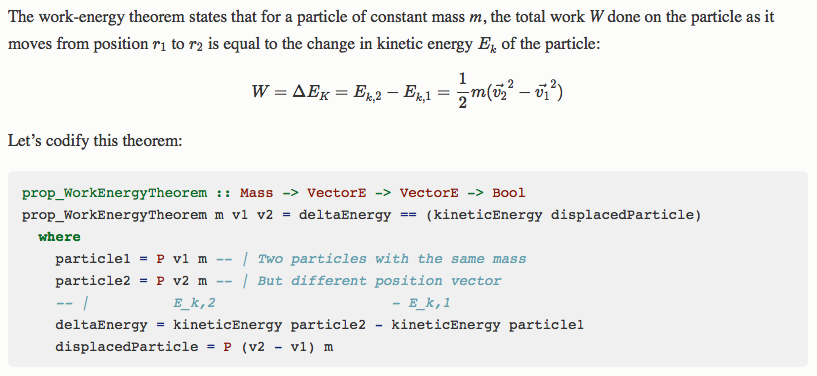
\includegraphics[width=1\textwidth]{figure/komposit-Ex.png}}
  \caption{Implementation av relationen arbete-energi i läromaterialet}
  \label{fig:komposit-ex}
\end{figure}

Implementation kan kompileras och testas och ska då visa på att
implementationerna av de grundläggande områdena är både rigorösa och korrekta.
Dessutom visar det att det går att använda det material som presenteras tidigare
till  att implementera och lösa mer komplexa problem.

\section{Skapande av och publicering på hemsidan}

Läromaterialet kompilerades med hjälp av ett bygg-skript och
publicerades på en internethemsida. Bygg-skriptet anropar
Pandoc för att konvertera från källkod och text i Literate
Haskell-formatet till HTML, redo att visas på en hemsida. Pandoc
paketerar även med \textit{MathJax} som använder JavaScript för att
rendera matematiska formler i LaTeX-format på fint och läsbart
vis. Utan stöd för JavaScript skrivs matematik ut som omodifierad
LaTeX-kod, vilket är mer svårläst, men fortfarande tolkningsbart. Det
skrevs även CSS-kod manuellt för att modifiera utseendet av
hemsidan så att den skulle bli prydligare och mer lättläst.

Varje källfil betraktades som ett kapitel och publicerades som en
separat undersida. Med hjälp av ett index beskrivet i bygg-skriptet
konstruerades navigationselement mellan kapitel på varje undersida
och en innehållsförteckning.

För publicering lades all data producerad av bygg-skriptet i en ny git-gren (engelska \textit{git branch}) med namnet \texttt{gh-pages}. Att alla grenar synkroniseras
mot GitHub medför att alla filer på \texttt{gh-pages} grenen
visas som en hemsida med hjälp av \textit{GitHub
  Pages}. Publiceringen skedde inte kontinuerligt eller automatiskt,
utan krävde en manuell synkronisering vid varje önskad uppdatering av
hemsidan.

\section{Utvärdering med testgrupp}

  % Återkoppling från examinator (NAD): "Nils Anders Danielsson <nad@cse.gu.se>
  % 27 Feb (1 day ago)
  % to Patrik, Andreas
  % Hi,Your BSc project groups both try to make tools for learning. I had some
  % discussion with Andreas' group about their plans for evaluating how well
  % their product works. My position is that, given the resource limits of
  % these projects (and general problems of reproducibility in social
  % sciences), it is very hard to perform an evaluation that gives useful
  % results. I don't mind if your groups try to perform some kind of
  % evaluation, but I suggest that you tell them to avoid overstating the
  % importance of the evaluations in the final reports."
  % Jag tror det är kompatibelt med det jag sagt tidigare - att göra en "ordentlig" utvärdering av det pedagogiska utfallet är komplicerat och tar (kalender-)tid.
  % Informell utvärdering av en testgrupp bör dock ingå.

För att utvärdera läromaterialet gjordes en kort och informell utvärdering med
en testgrupp. Testgruppen bestod av tre andra studenter på Chalmers som gick
tredje året på Datateknik eller Informationsteknik. De hade alla läst Fysik för
ingenjörer eller motsvarande sedan innan och de hade läst en kurs i Haskell.
Däremot hade de inte läst DSLsofMath eller motsvarande. Domänspecifika språk var
med andra ord nytt för dem.

Utvärderingen gjordes genom att visa dem läromaterialet och ge det en kort
presentation och bakgrund. Sedan fick de på egen hand läsa det. Deras spontana
reaktioner och svar på frågor noterades.

\section{Möten med fysikläraren}

För att få återkoppling på läromaterialet hölls två möten med Åke Fäldt,
föreläsare och examinator för Fysik för ingenjörer. Ett möte hölls relativt
tidigt i projektet, 2018-03-02, och ett andra relativt sent, 2018-04-11.
Under mötena presenterades läromaterialet i sig och tanken med det, nämligen att
presentera fysik på ur ett annat perspektiv, ett
programmeringsperspektiv. Det diskuterades också svåra områden i Fysik för
ingenjörer (se avsnitt \ref{sec:kontakt_faldt}), vad läromaterialet skulle kunna bidra med för kunskaper till
studenter samt dess eventuella roll i relation till fysikkursen i övrigt.
